\section{Classification: Generative and Discriminative}
\begin{itemize}
	\item Classification is a fundamentally different problem than a regression
		problem. IN a regression problem, we usually deal with a dataset \( y_i \in
		\R \), but in regression, the output is not a real number but rather a label:
		\[
			\mathcal{X} \to \mathcal{Y} \in \{0, \dots, K - 1\}
		\]
	\item The labels can be binary, or also perhaps more complicated. The MNIST
		dataset is not binary, since we have images and we want to classify them into
		the digits 0-9, for example. 
	\item In general, the problem is phrased like this: given a dataset \( \{(x_i,
		y_i)\}_{i = 1}^{n} \), we are interested in \textit{learning} the
		classification 
		\[
			f_{\theta}: \mathcal{X} \to \{0, \dots K - 1\}
		\]
\end{itemize}
\subsection{Bayes' Rule}
\begin{itemize}
	\item In the context of classification, it's used to transform class-conditional
		probabilities into posterior probabilities. In particular,
		\begin{align*}
			p(0 \mid x) &= \frac{p(x \mid 0) p(0)}{p(x)}\\
			p(1 \mid x) &=  \frac{p(x \mid 1) p(1)}{p(x)} 
		\end{align*}
		The variables \( p(x \mid 0), p(x \mid 1) \) are called the
		\textit{class-conditional probabitlities}. The value of \( p(x) \) is
		determined using the law of total probability:
		\[
			p(x) = p(x \mid 0) p(0) + p(x \mid 1) p(1)
		\]
	\item The hard part is finding the right class-conditional probability --
		we always have to ask ourselves, what kind of distribution do we expect? The
		answer to this is usually motivated by our prior knowledge about the
		population; maybe half of the population we expect to tend one way, so our
		distribution should reflect that. 
	\item If we map the posterior probabilities, we'll get a graph like this: 

		\begin{center}
			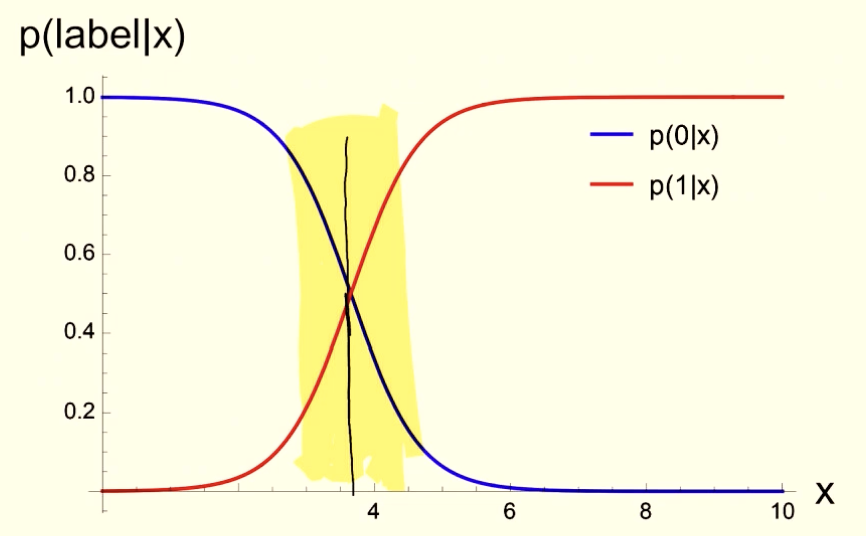
\includegraphics[scale=0.5]{lec-6a.png}
		\end{center}
		But what should we do in the region highlighted in yellow? This is a
		gray-area, where we aren't 100\% certain that we should classify one way or
		the other.     
		\begin{itemize}
			\item One thing we can do here is look at the intersection between these
				two curves, call it \( x^{*} \), and basically classify:
				\[
					f_{\theta}(x) = \begin{cases}
						0 & x < x^{*}\\
						1 & x \geq x^{*}
					\end{cases}
				\]
			\item This is a somewhat reasonable rule to follow, since this allows us
				to potentially reduce the probability of classifying incorrectly at
				least from a probabilistic standpoint.  
		\end{itemize}
	\item In general, we want to pick a value of \( k \) (the classification) 
		such that \( p(k \mid x) \)
		is maximal. Equivalently, this means that we want to reduce the probability
		of error:
		\[
			P(\text{error}) = \int p(\text{error}\mid x) p(x) \diff x 
		\]
		In doing this, you are treating false positives and false negatives with eual
		weight. However, this is not always the case. For instance, if you're in the
		medical field, false negatives can be much more detrimental than false
		positives, often fatal, so in cases like that we should be more careful about
		how we classify things.  

		\question{What if you just classify the error as the probability of
			\textit{misclassificaiton}? It seems that we're phrasing "error" in terms
		of testing positive, which isn't the best method of classification?}

		\comment{It seems like they haven't covered exactly how to quantify error
		just yet.} 
\end{itemize}

\subsection{Ways of Building Classifiers}
\begin{itemize}
	\item There are three main ways we can build classifiers: 
		\begin{enumerate}[label=\arabic*.]
			\item \textbf{Generative:} to model the conditional probabilities \( p(x
				\mid k)\), then use Bayes' rule to get \( p(k \mid x) \). This
				requires you to somehow model the prior \( p(k) \). 
			\item \textbf{Discriminative:} Model \( p(k \mid x) \) directly. 
			\item \textbf{Find Decision Boundaries:} Directly solve for the
				boundaries \( f : \mathcal{X} \to \{0, \dots, K - 1\} \).  

				This approach has the drawback that you lose information about how
				close your data point is to any of the boundaries, which means that
				you lose the ability to quantify your model's uncertainty in the
				system.  
		\end{enumerate}
\end{itemize}
\subsection{Logistic Regression}
\begin{itemize}
	\item Logistic regression is a classification method, where we model the
		posterior probability by a logistic function:
		\[
			p(k = 0 \mid x) = \frac{1}{1 + e^{-(\theta_1 x + \theta_0)}}
		\]
		We can also extend this to \( K \) classes, but for now we will talk about
		two classes 0 and 1.   
	\item If the class-conditional density \( p(x \mid \{0, 1\}) \) is Gaussian, then
		we claim that the posterior probability will be a logistic function 
		in \( z = \theta_1x + \theta_0 \). 

		\question{What is \( \theta_1, \theta_0 \)? Are these fitted parameters, or
		what?} 

		\answer{No, \( \theta_1 \) and \( \theta_0 \) are parameters that you can
			mathematically solve for. You can solve for these variables by literally
			letting \( P(x \mid k) \sim N(\mu_k, \sigma)\) (assume the variances are the
		same), and work out the math via Bayes' rule. }
	\item In our case then, \( z \) is a linear function of \( x \), plus a bias term
		\( \theta_0 \). This is called an "affine" function. 
	\item We can then generalize this to multivariate Gaussians, where we assume:
		\[
			P(X \mid k) \sim N(\mu_k, \Sigma)
		\]
		here \( \Sigma \) is the covariance matrix. 

		\comment{Review the proof in the slides, ask about what's happening.} 
	\item Intuitively, we want a sigmoid (logistic) function to model our
		probabilities because it's very nice -- the probability is always between 0
		and 1, so it's always well-behaved, and it's also smooth so there's nice
		properties there as well. 
\end{itemize}
\subsection{Modeling the Posterior Probability Distribution}
\begin{itemize}
	\item To give a preview, here's what we're going to do:

		We basically set up a label \( Y \in \{0, 1\} \) to be a Bernoulli random
		variable (for simplicity I think), with its probability parameter so we have:
		\[
			P(Y = 1 \mid x) = \frac{1}{1 + \exp(- \theta^{\top} x - \theta_0)} :=
			\mu(x)
		\]
	\item In the binary case, we can take \( y \) to denote the values taken on by
		the random variables, so:
		\[
			p(y \mid x) = \mu(x)^{y} (1 - \mu(x))^{1 - y}
		\]
		(this is just law of total probability applied to Bernoulli RVs). 
	\item In the next lecture, we will learn how to estimate \( \theta_1, \theta_0 \)
		using MLE methods. 
\end{itemize}
